\section{Method}
\label{sec:method}

ClothDojo separates physical trajectory generation from visual data expansion
(Fig.~\ref{fig:method-framework}). We first train NOCS-conditioned trajectory
agents from human demonstrations and corrections, then deploy them on unseen
garments and initial states. We automatically filter the resulting rollouts
using task metrics and re-render the successful ones under different appearances to train RGB
policies. One successful physical rollout can thus yield multiple visual
versions without regenerating its actions.

\subsection{Interaction environment and tasks}

ClothDojo combines MuJoCo robot dynamics~\cite{todorov2012mujoco} with Style3D
cloth simulation in Newton~\cite{newton} to support continuous bimanual
control. Virtual reality (VR) teleoperation and policy execution use the same
physics, so human
demonstrations, corrections, and autonomous rollouts share the same
robot--cloth interaction. Fig.~\ref{fig:folding-trajectories} shows
autonomous trajectories in which the agents repeatedly grasp, coordinate both
arms, and adjust their actions as the cloth state changes.

We convert more than 10,000 garments from the large-scale parametric
GarmentCodeData dataset~\cite{GarmentCodeData} into simulation assets and
select 500 structurally diverse garments for our experiments. As shown in
Fig.~\ref{fig:garment-assets}, this set spans large variations in garment
length, body width, sleeve length, and sleeve width, and includes sleeveless,
hooded, low-cut, open-back, asymmetric, and unconventional designs.

\begin{figure}[t]
  \centering
  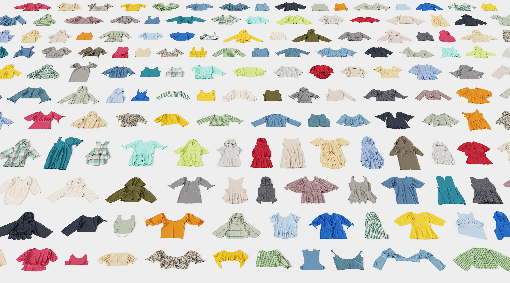
\includegraphics[width=\linewidth]{figures/clothdojo-garment-assets.pdf}
  \caption{\textbf{The experimental garment set spans diverse geometries.}
  The figure shows most of the 500 assets, covering different garment lengths,
  widths, sleeve types, necklines, and asymmetric cuts. All garments are
  naturally settled and shown at their relative physical sizes.}
  \label{fig:garment-assets}
\end{figure}

\textbf{Flattening} starts from a crumpled state produced by randomly hanging,
releasing, and settling a garment. The goal is a naturally flat, face-up
configuration. All four cardinal orientations on the table are accepted, and its
position within the tabletop is unconstrained. \textbf{Folding} starts from a
successful final state of the preceding flattening task. The goal is a compact,
flat rectangular bundle with little protruding material. We prescribe no
aspect ratio, crease pattern, or action order. Initial states for both tasks
are saved in advance so that policies can run from identical states; the
quantitative success criteria are given in Sec.~\ref{sec:success-criteria}.

\subsection{NOCS-conditioned trajectory agents}

We provide a surface-position reference that remains consistent as the cloth
deforms by encoding normalized object coordinate space
(NOCS)~\cite{wang2019nocs} as the garment texture. Let $v_i$ denote a vertex
of the canonical mesh, with component-wise bounds $v_{\min}$ and $v_{\max}$.
Its normalized coordinate is
\begin{equation}
  u_i=\frac{v_i-v_{\min}}{v_{\max}-v_{\min}},
  \label{eq:nocs-color}
\end{equation}
whose three components form the RGB channels. Each color is assigned in the
canonical configuration and remains attached to the corresponding vertex as
the garment deforms. Similar relative positions across garments therefore
receive similar colors. This exposes canonical surface-position cues through
the model's existing image interface. The agent still observes only visible
surfaces, and matching colors do not imply exact semantic correspondence
across garments.

We use the pretrained $\pi_{0.5}$ model~\cite{pi05} as the base and separately
fine-tune trajectory agents for flattening and folding. Each agent receives
NOCS images through the model's original visual interface, together with the
robot state and task instruction, and predicts joint targets and gripper
commands for both arms. During execution, the agent applies only a prefix of
each predicted action sequence and then replans from the latest observation,
producing a closed-loop trajectory.

\subsection{Learning from demonstrations and corrections}
\label{sec:experience-corrections}

We collect separate flattening and folding demonstrations through VR
teleoperation. To collect a folding demonstration, we restore the final state
of its corresponding flattening demonstration and continue from that state.
The tasks are recorded separately and used to fine-tune their respective
agents with the base model's action-prediction objective. Sec.~\ref{sec:trajectory-agent-eval}
reports the garment coverage and number of demonstrations.

To cover states induced by the agents themselves, we use DAgger-like iterative
data aggregation~\cite{DAgger}. Each agent first rolls out autonomously on
different garments and initial states. For an execution that requires
correction, an operator selects an intervention point, restores that simulation
state, and continues the task through VR, producing a correction trajectory
$\mathcal D_H$. We then combine these corrections with the original
demonstrations $\mathcal D_E$ and update the agent using the same supervised
objective. All supervised actions are provided by humans; at this stage,
autonomous rollouts supply the starting states for correction.

To add training examples with exchanged arm roles, we apply bilateral
morphological symmetry augmentation~\cite{GR-RL} to every human trajectory.
At each frame, we reflect the garment state and transform the robot states and
actions while exchanging the two arms and grippers. We then re-render NOCS
observations by replaying the transformed states. Each human trajectory yields
one mirrored sample, which is not counted as an additional human demonstration.

\subsection{RGB data from successful trajectories}

After training, we freeze the trajectory agents and roll them out
autonomously on unseen garments and initial states. The task criteria in
Sec.~\ref{sec:success-criteria} automatically filter the results, retaining only
successful trajectories.

For each successful trajectory, we sample from 34 base garment materials with
39 color variants, 17 table materials, 12 floor materials, and eight
background scenes. Light position, intensity, and color temperature are drawn
from continuous ranges. Each appearance remains fixed within a trajectory. We
replay the saved states to render RGB observations while preserving the robot
and garment motion, robot states, and action targets. The resulting data train
downstream policies that receive RGB observations, robot states, and task
instructions without NOCS. A physical trajectory may produce multiple visual
versions, but we count it as one manipulation experience. The appearance
subsets used for training and evaluation are specified in the experimental
setup.
